\pdfoutput=1
\documentclass[a4paper,pdflatex,ja=standard]{bxjsarticle}

% ---Setting about the geometry of the document----
% \usepackage{a4wide}
% \pagestyle{empty}

% ---Physics and Math Packages---
\usepackage{amssymb,amsfonts,amsthm,mathtools}
\usepackage{physics,braket,bm}

% ---underline---
\usepackage{ulem}

% --- sorround the texts or equations
% \usepackage{fancybox,ascmac}

% ---settings of theorem environment---
% \usepackage{amsthm}
% \theoremstyle{definition}

% ---settings of proof environment---
% \renewcommand{\proofname}{\textbf{証明}}
% \renewcommand{\qedsymbol}{$\blacksquare$}

% ---Ignore the Warnings---
\usepackage{silence}
\WarningFilter{latexfont}{Some font shapes,Font shape}

% ---Insert the figure (If insert the `draft' at the option, the process becomes faster)---
% \usepackage{graphicx}
% \usepackage{subcaption}

% ----Add a link to a text---
\usepackage{url}
\usepackage{xcolor,hyperref}
\hypersetup{colorlinks=true,citecolor=orange,linkcolor=blue,urlcolor=magenta}
\usepackage{bxcjkjatype}

% ---Tikz---
\usepackage{tikz,pgf,pgfplots,circuitikz}
\pgfplotsset{compat=1.15}
\usetikzlibrary{intersections,arrows.meta,angles,calc,3d,decorations.pathmorphing}

% ---Add the section number to the equation, figure, and table number---
\makeatletter
   \renewcommand{\theequation}{\thesection.\arabic{equation}}
   \@addtoreset{equation}{section}
   
   \renewcommand{\thefigure}{\thesection.\arabic{figure}}
   \@addtoreset{figure}{section}
   
   \renewcommand{\thetable}{\thesection.\arabic{table}}
   \@addtoreset{table}{section}
\makeatother

% ---enumerate---
% \renewcommand{\labelenumi}{$\arabic{enumi}.$}
% \renewcommand{\labelenumii}{$(\arabic{enumii})$}

% ---Index---
% \usepackage{makeidx}
% \makeindex 

% ---Title---
\title{Tikz サンプル}
\author{宮根一樹}
\date{\today}

\begin{document}

\maketitle

\begin{figure}[ht]
  \centering    
  \begin{tikzpicture}[scale=2.0]  
      \draw[->,>=stealth,ultra thin](-1,0)--(2,0)node[above right]{$\varepsilon$};
      \draw[->,>=stealth,thin](0,-0.5)--(0,1.5)node[right]{$f(\varepsilon)$};
      \draw[dashed,ultra thin](-1,1)--(2,1);
      \draw[dotted,thin](1,1/2)--(1,0)node[below]{$\mu$};
      \draw[dotted,thin](1,1/2)--(0,1/2)node[left]{$\frac{1}{2}$};
      \draw(0,0)node[below left]{O};
      \draw(0,1)node[above left]{$1$};
      \draw[thick,samples=100,domain=-1:1.22]plot(\x,{1/(exp(36*(\x-1))+1)});    
    \end{tikzpicture}    
    \caption{$f(\varepsilon)$の概略図}
\end{figure}

\begin{figure}[ht]
  \centering    
  \begin{tikzpicture}[scale=2.0]  
      \draw[->,>=stealth,ultra thin](-2.5,0)--(2.5,0)node[above right]{$\varepsilon$};
      \draw[->,>=stealth,thin](0,-0.5)--(0,1.5);
      \draw(0,0)node[below left]{O};
      \draw(0,1)node[above left]{$1$};
      \draw[thick,samples=100,domain=0:1.3,dotted,thin]plot(\x,{1/(exp(20*(\x-1))+1)});
      \draw[thick,samples=100,domain=-1.3:0,dotted,thin]plot(\x,{1/(exp(20*(-\x-1))+1)});  
      \draw[thick,samples=100,domain=-1/2:1.3-1/2,red,thick]plot(\x,{1/(exp(20*((\x+1/2)-1))+1)});
      \draw[thick,samples=100,domain=-1.3-1/2:-1/2,red,thick]plot(\x,{1/(exp(20*(-(\x+1/2)-1))+1)});
      \draw(-1.5,1)node[above left]{$g(\bm{k},t+\delta t)$};
    \end{tikzpicture}
    \caption{$g(\bm{k},t+\delta t)$と$g^{0}(\bm{k},t)$の概略図}
\end{figure}

\begin{figure}[ht]
  \centering    
  \begin{tikzpicture}[scale=1.5] 
    \draw[->,>=stealth,ultra thin](-0.2,0)--(3,0)node[below]{$T$};
    \draw[->,>=stealth,thin](0,-0.5)--(0,2.0)node[right]{$c$};
    \draw[dashed,ultra thin](-0.2,1.8)--(3,1.8);
    \draw(0,0)node[below left]{O};
    \draw(0,1.8)node[below left]{$3nk_B$};
    \draw[dotted,samples=100,domain=-0.2:1.3]plot(\x,\x^3)node[right]{$T^3$};
    \draw[samples=100,domain=-0.2:3]plot(\x,{1.8/(1+exp(-(4*\x-4.6)))});
  \end{tikzpicture}    
  \caption{比熱$c$の概略図}
\end{figure}

\begin{figure}[ht]
  \centering    
  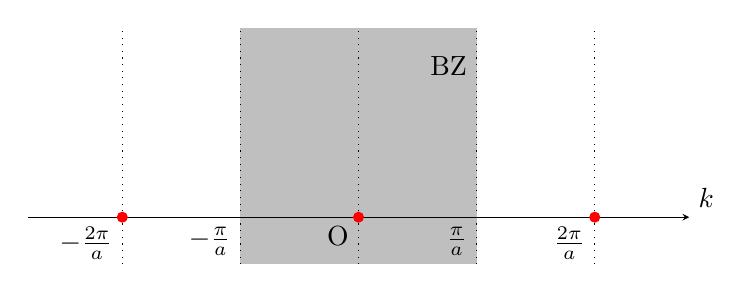
\begin{tikzpicture}
    \begin{scope}[xscale = 1.5, yscale = 1.2]
      \fill[lightgray](-1,-0.5)--(-1,2)--(1,2)--(1,-0.5)--cycle;
      \draw[dotted,thin](0,-0.5)--(0,2);
      \draw[->,>=stealth,ultra thin](-2.8,0)--(2.8,0)node[above right]{$k$};
      \draw[dotted,thin](1,-0.5)--(1,2);
      \draw[dotted,thin](-1,-0.5)--(-1,2);
      \draw[dotted,thin](2,-0.5)--(2,2);
      \draw[dotted,thin](-2,-0.5)--(-2,2);
      \draw(0,0)node[below left]{O};
      \draw(1,0)node[below left]{$\frac{\pi}{a}$};
      \draw(1,1.8)node[below left]{BZ};
      \draw(-1,0)node[below left]{$-\frac{\pi}{a}$};
      \draw(2,0)node[below left]{$\frac{2\pi}{a}$};
      \draw(-2,0)node[below left]{$-\frac{2\pi}{a}$};
    \end{scope}					        
    \fill[red](3,0)circle[radius=2pt];
    \fill[red](-3,0)circle[radius=2pt];
    \fill[red](0,0)circle[radius=2pt];
    \end{tikzpicture}    
    \caption{逆格子と第1ブリルアンゾーン}
\end{figure}

\begin{figure}[ht]
  \centering    
  \begin{tikzpicture}[scale=1.5] 
      \draw[->,>=stealth,ultra thin](0,-0.5)--(0,3.2)node[above right]{$\varepsilon$};
      \draw[->,>=stealth,ultra thin](-2.8,0)--(2.8,0)node[above right]{$k$};
      \draw[dotted,thin](1,-0.5)--(1,3.2);
      \draw[dotted,thin](-1,-0.5)--(-1,3.2);
      \draw[dotted,thin](2,-0.5)--(2,3.2);
      \draw[dotted,thin](-2,-0.5)--(-2,3.2);
      \draw(0,0)node[below left]{O};
      \draw(1,0)node[below left]{$\frac{\pi}{a}$};
      \draw(-1,0)node[below left]{$-\frac{\pi}{a}$};
      \draw(2,0)node[below left]{$\frac{2\pi}{a}$};
      \draw(-2,0)node[below left]{$-\frac{2\pi}{a}$};
      \draw[samples=100,domain=-2.8:2.8,ultra thin,dashed]plot(\x,{0.5*(\x*\x)/2.4});
      \draw[samples=100,domain=-1.0:1.0,thick,red]plot(\x,{0.5*((\x)^2)/2.4});
      \draw[samples=100,domain=-1.0:0,thick,red]plot(\x,{0.5*((\x+2)^2)/2.4});
      \draw[samples=100,domain=0:1.0,thick,red]plot(\x,{0.5*((\x-2)^2)/2.4});
      \draw[samples=100,domain=-1.0:0,thick,red]plot(\x,{0.5*((\x-2)^2)/2.4});
      \draw[samples=100,domain=0:1.0,thick,red]plot(\x,{0.5*((\x+2)^2)/2.4});
      \begin{scope} \clip (-2.8,-0.5) rectangle (2.8,3.2);
        \draw[samples=100,domain=-1.0:0,thick,red]plot(\x,{0.5*((\x+4)^2)/2.4});
        \draw[samples=100,domain=0:1.0,thick,red]plot(\x,{0.5*((\x-4)^2)/2.4});
      \end{scope}
    \end{tikzpicture}    
    \caption{自由粒子の分散関係}
\end{figure}

\begin{figure}[ht]
  \centering    
  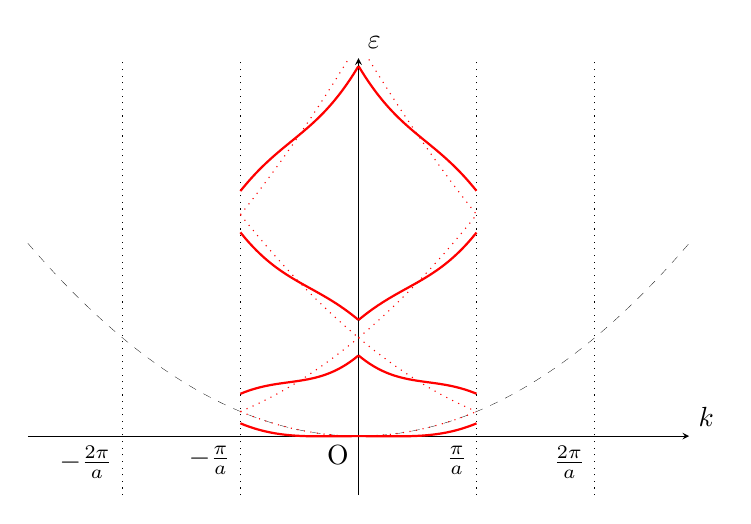
\begin{tikzpicture}[scale=1.5] 
    \draw[->,>=stealth,ultra thin](0,-0.5)--(0,3.2)node[above right]{$\varepsilon$};
    \draw[->,>=stealth,ultra thin](-2.8,0)--(2.8,0)node[above right]{$k$};
    \draw[dotted,thin](1,-0.5)--(1,3.2);
    \draw[dotted,thin](-1,-0.5)--(-1,3.2);
    \draw[dotted,thin](2,-0.5)--(2,3.2);
    \draw[dotted,thin](-2,-0.5)--(-2,3.2);
    \draw(0,0)node[below left]{O};
    \draw(1,0)node[below left]{$\frac{\pi}{a}$};
    \draw(-1,0)node[below left]{$-\frac{\pi}{a}$};
    \draw(2,0)node[below left]{$\frac{2\pi}{a}$};
    \draw(-2,0)node[below left]{$-\frac{2\pi}{a}$};
    \draw[samples=100,domain=-2.8:2.8,ultra thin,dashed]plot(\x,{0.5*(\x*\x)/2.4});\draw[samples=100,domain=-1.0:1.0,thin,red,dotted]plot(\x,{0.5*((\x)^2)/2.4});
    \draw[samples=100,domain=-1.0:0,thin,red,dotted]plot(\x,{0.5*((\x+2)^2)/2.4});
    \draw[samples=100,domain=0:1.0,thin,red,dotted]plot(\x,{0.5*((\x-2)^2)/2.4});
    \draw[samples=100,domain=-1.0:0,thin,red,dotted]plot(\x,{0.5*((\x-2)^2)/2.4});
    \draw[samples=100,domain=0:1.0,thin,red,dotted]plot(\x,{0.5*((\x+2)^2)/2.4});
    \begin{scope} \clip (-2.8,-0.5) rectangle (2.8,3.2);
      \draw[samples=100,domain=-1.0:0,thin,red,dotted]plot(\x,{0.5*((\x+4)^2)/2.4});
      \draw[samples=100,domain=0:1.0,thin,red,dotted]plot(\x,{0.5*((\x-4)^2)/2.4});
    \end{scope}
    \draw[samples=100,domain=-1.0:1.0,thick,red]plot(\x,{0.5*((\x)^2)/2.4-0.1*(sin(\x*90))^2});
    \draw[samples=100,domain=-1.0:0,thick,red]plot(\x,{0.5*((\x+2)^2)/2.4+0.15*sin((\x-0.5)*180)});
    \draw[samples=100,domain=0:1.0,thick,red]plot(\x,{0.5*((\x-2)^2)/2.4-0.15*sin((\x+0.5)*180)});
    \draw[samples=100,domain=-1.0:0,thick,red]plot(\x,{0.5*((\x-2)^2)/2.4-0.15*sin((\x-0.5)*180)});
    \draw[samples=100,domain=0:1.0,thick,red]plot(\x,{0.5*((\x+2)^2)/2.4+0.15*sin((\x+0.5)*180)});
    \begin{scope} \clip (-2.8,-0.5) rectangle (2.8,3.2);
      \draw[samples=100,domain=-1.0:0,thick,red]plot(\x,{0.5*((\x+4)^2)/2.4+0.2*sin((\x-0.5)*180)});
      \draw[samples=100,domain=0:1.0,thick,red]plot(\x,{0.5*((\x-4)^2)/2.4-0.2*sin((\x+0.5)*180)});
    \end{scope}
  \end{tikzpicture}    
    \caption{弱い周期ポテンシャル中のの分散関係}
\end{figure}

\begin{figure}[ht]
  \centering    
  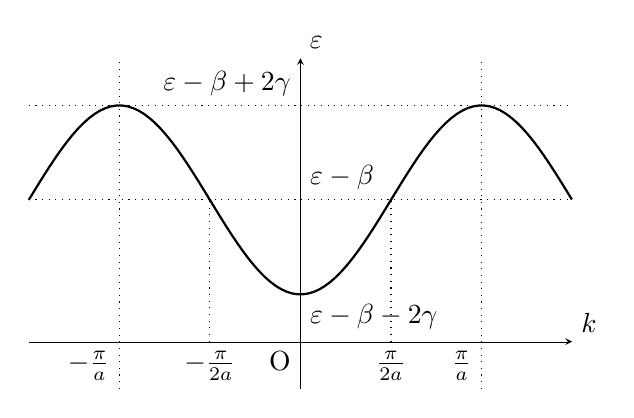
\begin{tikzpicture}[xscale = 2.3, yscale = 1.2] 
      \draw[->,>=stealth,ultra thin](0,-0.5)--(0,3)node[above right]{$\varepsilon$};
      \draw[->,>=stealth,ultra thin](-1.5,0)--(1.5,0)node[above right]{$k$};
      \draw[dotted,thin](1,-0.5)--(1,3);
      \draw[dotted,thin](-1,-0.5)--(-1,3);
      \draw[dotted,thin](-1.5,2.5)--(1.5,2.5);
      \draw[dotted,thin](-1.5,1.5)--(1.5,1.5);
      \draw[dotted,thin](1/2,0)--(1/2,1.5);
      \draw[dotted,thin](-1/2,0)--(-1/2,1.5);
      \draw(0,0)node[below left]{O};
      \draw(1,0)node[below left]{$\frac{\pi}{a}$};
      \draw(-1,0)node[below left]{$-\frac{\pi}{a}$};
      \draw(1/2,0)node[below]{$\frac{\pi}{2a}$};
      \draw(-1/2,0)node[below]{$-\frac{\pi}{2a}$};
      \draw(0,0.5)node[below right]{$\varepsilon-\beta-2\gamma$};
      \draw(0,2.5)node[above left]{$\varepsilon-\beta+2\gamma$};
      \draw(0,1.5)node[above right]{$\varepsilon-\beta$};
      \draw[samples=100,domain=-1.5:1.5,thick]plot(\x,{1.5-cos(\x*180)});
    \end{tikzpicture}
    \caption{$\varepsilon(k)$の概略図}
\end{figure}

\begin{figure}[ht]
  \centering    
  \begin{tikzpicture}
    \begin{scope}[xscale = 2.3, yscale = 1.2] 
      \draw[->,>=stealth,ultra thin](0,-0.5)--(0,3);
      \draw[->,>=stealth,ultra thin](-1.5,0)--(1.5,0)node[above right]{$x$};
      \draw[dotted,thin](1,-0.5)--(1,3);
      \draw[dotted,thin](-1,-0.5)--(-1,3);
      \draw(0,0)node[below left]{O};
      \draw(1,0)node[below left]{$a$};
      \draw(-1,0)node[below left]{$a$};
      \draw[samples=100,domain=-1:1,thick]plot(\x,{2.4*(cos(\x*90))^8});          
    \end{scope}        
    \fill[red](2.3,0)circle[radius=2pt];
    \fill[red](-2.3,0)circle[radius=2pt];
    \fill[red](0,0)circle[radius=2pt];
  \end{tikzpicture}
    \caption{$\varphi(x)$の概略図}
\end{figure}

\begin{figure}[ht]
  \centering    
  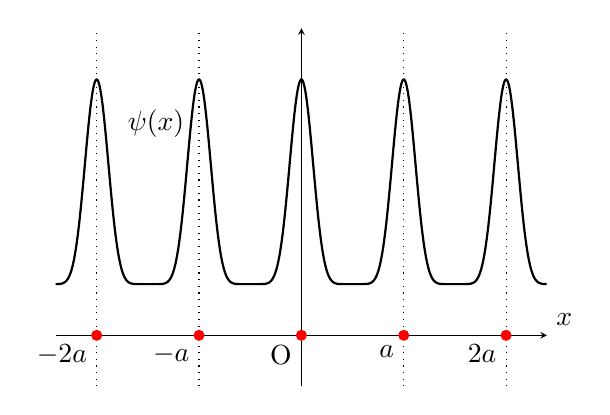
\begin{tikzpicture}
    \begin{scope}[scale=1.3] 
      \draw[->,>=stealth,ultra thin](0,-0.5)--(0,3);
      \draw[->,>=stealth,ultra thin](-2.4,0)--(2.4,0)node[above right]{$x$};
      \draw[dotted,thin](1,-0.5)--(1,3);
      \draw[dotted,thin](-1,-0.5)--(-1,3);          
      \draw[dotted,thin](2,-0.5)--(2,3);
      \draw[dotted,thin](-2,-0.5)--(-2,3);
      \draw(0,0)node[below left]{O};
      \draw(1,0)node[below left]{$a$};
      \draw(-1,0)node[below left]{$-a$};
      \draw(2,0)node[below left]{$2a$};
      \draw(-2,0)node[below left]{$-2a$};
      \draw(-1.05,2.3)node[below left]{$\psi(x)$};
      \draw[samples=1000,domain=-2.4:2.4,thick]plot(\x,{2*(cos(\x*180))^8+0.5});          
    \end{scope}        
    \fill[red](1.3,0)circle[radius=2pt];
    \fill[red](-1.3,0)circle[radius=2pt];        
    \fill[red](0,0)circle[radius=2pt];        
    \fill[red](2.6,0)circle[radius=2pt];
    \fill[red](-2.6,0)circle[radius=2pt];  
  \end{tikzpicture}
    \caption{$k=0$のときの$\psi(x)$の概略図}
\end{figure}

\begin{figure}[ht]
  \centering    
  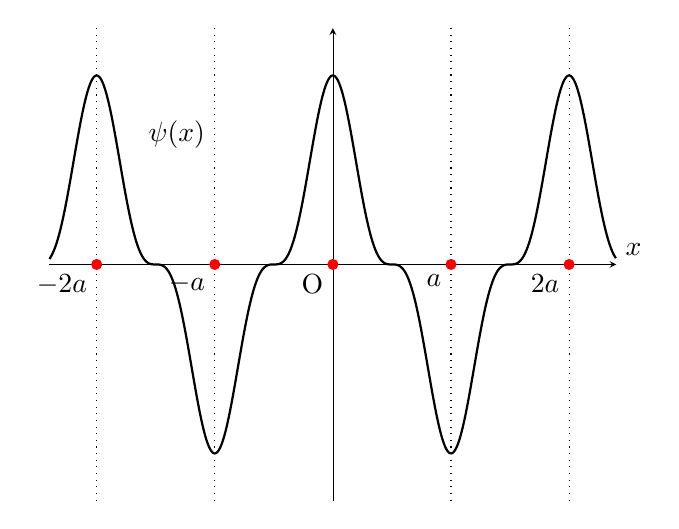
\begin{tikzpicture}
    \begin{scope}[scale=1.5] 
      \draw[->,>=stealth,ultra thin](0,-2)--(0,2);
      \draw[->,>=stealth,ultra thin](-2.4,0)--(2.4,0)node[above right]{$x$};
      \draw[dotted,thin](1,-2)--(1,2);
      \draw[dotted,thin](-1,-2)--(-1,2);          
      \draw[dotted,thin](2,-2)--(2,2);
      \draw[dotted,thin](-2,-2)--(-2,2);
      \draw(0,0)node[below left]{O};
      \draw(1,0)node[below left]{$a$};
      \draw(-1,0)node[below left]{$-a$};
      \draw(2,0)node[below left]{$2a$};
      \draw(-2,0)node[below left]{$-2a$};
      \draw(-1,1.3)node[below left]{$\psi(x)$};
      \draw[samples=1000,domain=-2.4:2.4,thick]plot(\x,{1.6*(cos(\x*180))^3});          
    \end{scope}        
    \fill[red](1.5,0)circle[radius=2pt];
    \fill[red](-1.5,0)circle[radius=2pt];        
    \fill[red](0,0)circle[radius=2pt];        
    \fill[red](3.0,0)circle[radius=2pt];
    \fill[red](-3.0,0)circle[radius=2pt];  
  \end{tikzpicture}
    \caption{$k=\pi/a$のときの$\psi(x)$の概略図}
\end{figure}

\begin{figure}[ht]
  \centering    
  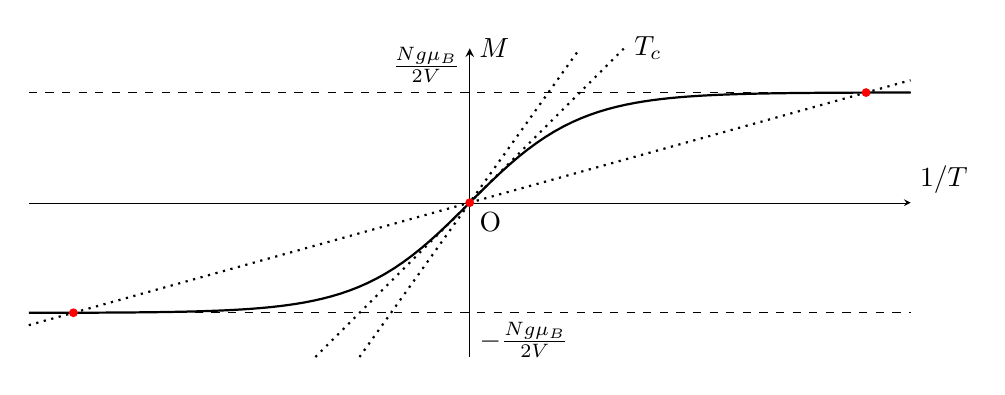
\begin{tikzpicture}[scale=1.4]
      \draw[->,>=stealth,ultra thin](-4,0)--(4,0)node[above right]{$1/T$};
      \draw[->,>=stealth,thin](0,-1.4)--(0,1.4)node[right]{$M$};
      \draw(0,0)node[below right]{O};
      \draw[dashed,thin](-4,1)--(4,1);
      \draw[dashed,thin](-4,-1)--(4,-1);
      \draw(0,1)node[above left]{$\frac{Ng\mu_{B}}{2V}$};          
      \draw(0,-1)node[below right]{$-\frac{Ng\mu_{B}}{2V}$};
      \draw[thick,samples=100,domain=-4:4,name path=A]plot(\x,{(exp(\x)-exp(-\x))/(exp(\x)+exp(-\x))});
      \draw[thick,samples=100,domain=-1.4:1.4,dotted]plot(\x,{\x})node[right]{$T_c$};
      \draw[thick,samples=100,domain=-1:1,dotted]plot(\x,{1.4*\x});
      \draw[thick,samples=100,domain=-4:4,name path=B,dotted]plot(\x,{\x/3.6});
      \path[name intersections={of= A and B, by={C,D,E}}];
      \fill[red](C)circle(0.04);
      \fill[red](D)circle(0.04);          
      \fill[red](E)circle(0.04);
    \end{tikzpicture}    
    \caption{$M$と$1/T$の関係}
\end{figure}

\begin{figure}[ht]
  \centering    
  \begin{tikzpicture}[scale=1.5] 
      \draw[->,>=stealth,thick](0,0)--(3,0)node[below]{$\bm{k}$};
      \draw[dotted,thin](-0.8,0)--(4.3,0)node[below]{$z$};
      \draw[->,>=stealth,thick](0,0)--({1.5*sqrt(3)},1.5)node[above left]{$\bm{k}'$};
      \draw[thin](3,0)--({1.5*sqrt(3)},1.5);
      \draw({1.5*sqrt(3)/2+1.44},1.5/2+0.3)node[right]{$q$};
      \draw [->,thin](0.7,0) arc (0:30:0.7);
      \draw(0.7,0.15)node[right]{$\theta$};
    \end{tikzpicture}    
    \caption{$q^2=|\bm{k}'-\bm{k}|^2$の関係}
\end{figure}

\begin{figure}[ht]
  \centering
  \begin{tikzpicture}

  \draw[-stealth](0,0,0) -- (3.5,0,0) node[right]{$y$};
  \draw[-stealth](0,0,0) -- (0,3.5,0) node[above]{$z$};
  \draw[-stealth](0,0,0) -- (0,0,6) node[below]{$x$};%\draw (0,0,0) node[below right]{O};

  \draw[- stealth,very thick](0,0,0) -- (3,3,3) node[right]{$\bm{n}$};
  \draw[dashed,thick](0,0,0) -- (3,0,3);
  \draw[dashed,thick](3,3,3) -- (3,0,3);
  
  \draw[- stealth,very thick](0,0,0) -- ({sqrt(2)},0,5) node[right]{$\bm{\epsilon}$};

  \draw[stealth - stealth](0,2,0) to[bend left] (3/2,3/2,3/2);
  \draw(0.8,1.9,0) node{$\theta$};

  \draw[stealth - stealth](1,1,1) to[bend left] ({sqrt(2)/3},0,5/3);
  \draw(0.42,-0.5,0) node{$\Theta$};

  \draw[stealth - stealth](0,0,{sqrt(27)/2}) to[bend right] (3/2,0,3/2);
  \draw(0.35,-1.3,0) node{$\phi$};

  \draw[stealth - stealth](0,0,{sqrt(27)*2.3/3}) to[bend right] ({sqrt(2)/3*2.3},0,5/3*2.3);
  \draw(-0.9,-2,0) node{$\psi$};
  
  \end{tikzpicture}
  \caption{$\bm{n}$と$\bm{\epsilon}$の取り方}
\end{figure}

\begin{figure}[ht]  
  \newcommand{\ctext}[1]{\raise0.2ex\hbox{\textcircled{\scriptsize{#1}}}}
  \centering
  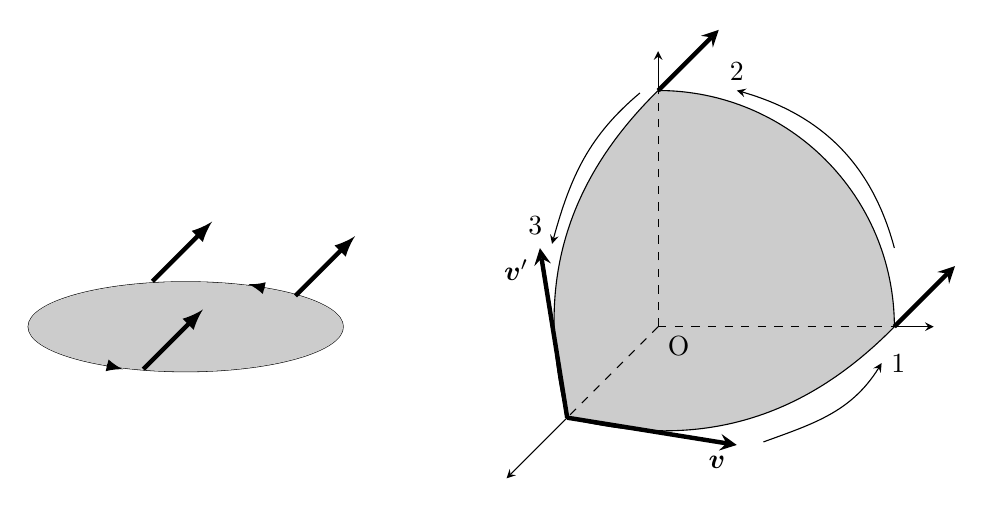
\begin{tikzpicture}
  
  \fill[black!20](0,3,0) to[out=0,in=90] (3,0,0) to[bend left] (0,0,3) to[bend left] (0,3,0);
  \draw(0,3,0) to[out=0,in=90] (3,0,0) to[bend left] (0,0,3) to[bend left] (0,3,0);

  \draw(-6,0,0) ellipse (2 and 0.57);
  \fill[black!20](-6,0,0) ellipse (2 and 0.57);  
  \draw[-latex,line width=1pt](1-6,0.49,0)--(0.8-6,0.54,0);
  \draw[-latex,line width=1pt](-1-6,-0.49,0)--(-0.8-6,-0.54,0);
  \draw[-latex, ultra thick](-6,0,1.4) -- (-6,0,-0.57);
  \draw[-latex, ultra thick](-6+1,0,1.4-2.42) -- (-6+1,0,-0.57-2.42);
  \draw[-latex, ultra thick](-6-1,0,1.4-2.9) -- (-6-1,0,-0.57-2.9);
  
  \draw[-stealth,ultra thick](0,0,3) -- (2.5,0,3.9) node[below left]{$\bm{v}$};
  \draw[-stealth,ultra thick](0,0,3) -- (0,2.5,3.9) node[below left]{$\bm{v}'$};

  \draw[-stealth,ultra thick](3,0,0) -- (3,0,-2);
  \draw[-stealth,ultra thick](0,3,0) -- (0,3,-2);

  \draw(3,1,0)[-stealth] to[out=105,in=345] (1,3,0) node[above]{$\ctext{2}$};
  \draw(2.8,0,3.8)[-stealth] to[out=20,in=240] (3.3,0,1.2) node[right]{$\ctext{1}$};  
  \draw(0,3.2,0.6)[-stealth] to[out=220,in=75] (0,2.4,3.5) node[above left]{$\ctext{3}$};
  
  \draw[dashed](0,0,0) -- (3,0,0);
  \draw[-stealth](3,0,0) -- (3.5,0,0);
  
  \draw[dashed](0,0,0) -- (0,3,0);
  \draw[-stealth](0,3,0) -- (0,3.5,0);
  
  \draw[dashed](0,0,0) -- (0,0,3);
  \draw[-stealth](0,0,3) -- (0,0,5);
  
  \draw (0,0,0) node[below right]{O};
  
  \end{tikzpicture}
  \caption{曲がった面の例}
\end{figure}

\begin{figure}[ht]
  \centering    
  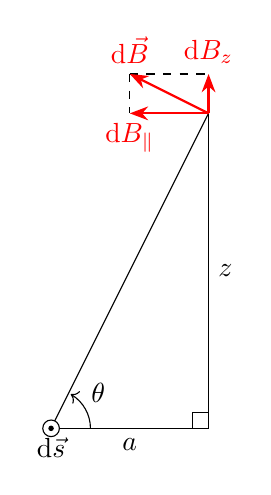
\begin{tikzpicture}
    \draw[thin](0,0)--(2,4);
    \draw[thin](0,0)--(2,0);
    \draw[thin](2,0)--(2,4);
    \draw[thin,dashed](1,4.5)--(2,4.5);      
    \draw[thin,dashed](1,4.5)--(1,4);
    \filldraw [fill=white] (0,0) circle [radius=3pt];
    \fill [fill=black] (0,0)circle [radius=1pt];
    \draw (0,0)node[below]{$\dd \vec{s}$};      
    \draw (1,0)node[below]{$a$};
    \draw (2,2)node[right]{$z$};
    \draw[thick,color=red,-Stealth](2,4)--(1,4.5)node[above]{$\dd \vec{B}$};
    \draw[thick,color=red,-Stealth](2,4)--(1,4)node[below]{$\dd B_{\parallel}$};
    \draw[thick,color=red,-Stealth](2,4)--(2,4.5)node[above]{$\dd B_{z}$};      
    \draw[thin](2,0.2)--(1.8,0.2)--(1.8,0);
    \draw [->](0.5,0) arc [start angle = 0, end angle = 60, radius = 0.5];
    \draw (0.6,0.2)node[above]{$\theta$};
  \end{tikzpicture}
  \caption{$\vec{r}-\vec{s}$と$\dd\vec{B}$の作る断面}    
\end{figure}

\begin{figure}[ht]
  \centering
    \begin{tabular}{cc}      
      \begin{minipage}[t]{0.3\linewidth}
        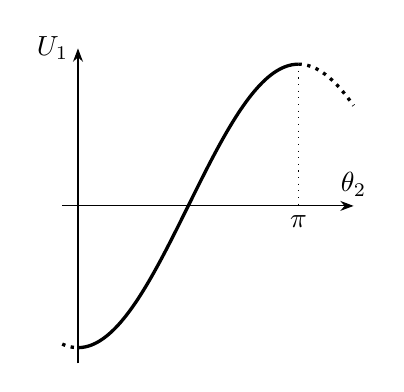
\begin{tikzpicture}
           \draw[thin,-Stealth] (-0.2,0)--(3.5,0)node[above]{$\theta_{2}$};
           \draw[thin,-Stealth] (0,-2)--(0,2)node[left]{$U_{1}$};
           \draw[very thick,samples=100,domain=-0:2.8]plot(\x,{-1.8*cos(\x*180/2.8)});
           \draw[very thick,samples=100,domain=-0.2:0,dotted]plot(\x,{-1.8*cos(\x*180/2.8)});
           \draw[very thick,samples=100,domain=2.8:3.5,dotted]plot(\x,{-1.8*cos(\x*180/2.8)});
           \draw [thin,dotted](2.8,1.8)--(2.8,0)node[below]{$\pi$};
        \end{tikzpicture}
        \caption{$\theta_{1}=0$のとき}
      \end{minipage} &
      \begin{minipage}[t]{0.3\linewidth}
        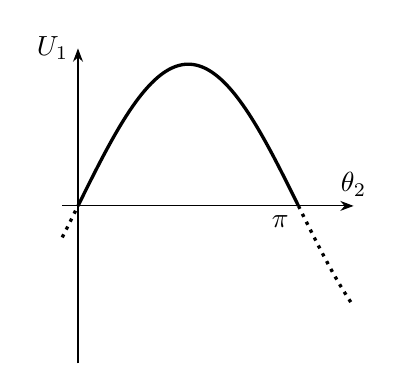
\begin{tikzpicture}
          \draw[thin,-Stealth] (-0.2,0)--(3.5,0)node[above]{$\theta_{2}$};
          \draw[thin,-Stealth] (0,-2)--(0,2)node[left]{$U_{1}$};
          \draw[very thick,samples=100,domain=-0:2.8]plot(\x,{1.8*sin(\x*180/2.8)});
          \draw[very thick,samples=100,domain=-0.2:0,dotted]plot(\x,{1.8*sin(\x*180/2.8)});
          \draw[very thick,samples=100,domain=2.8:3.5,dotted]plot(\x,{1.8*sin(\x*180/2.8)});
          \draw (2.8,0)node[below left]{$\pi$};
       \end{tikzpicture}  
      \caption{$\theta_{1}=\pi/2$のとき}
    \end{minipage}
  \end{tabular}
\end{figure}

\begin{figure}[ht]
  \centering    
  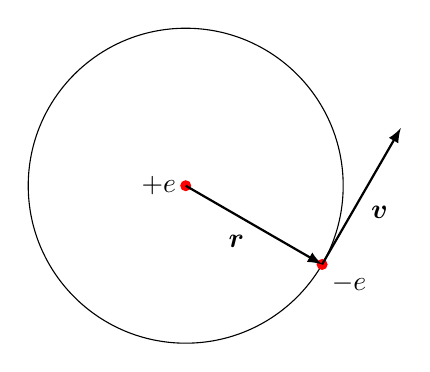
\begin{tikzpicture}[scale=1] 
      \draw (0,0) circle (2);
      \fill [color=red] ({sqrt(3)},-1) circle (2pt);      
      \fill [color=red] (0,0) circle (2pt);
      \draw (0,0) node [left]{$+e$};
      \draw[-latex,thick] ({sqrt(3)},-1)--({sqrt(3)+1},{-1+1*sqrt(3)});
      \draw[-latex,thick] (0,0)--({sqrt(3)},-1);
      \draw({sqrt(3)/2},-1/2)node [below left]{$\bm{r}$};
      \draw ({sqrt(3)},-1) node [below right]{$-e$};
      \draw ({sqrt(3)+0.5},{-1+0.5*sqrt(3)}) node [below right]{$\bm{v}$};
    \end{tikzpicture}    
    \caption{古典論におけるラザフォード原子模型}
\end{figure}

\begin{figure}[ht]
  \centering    
  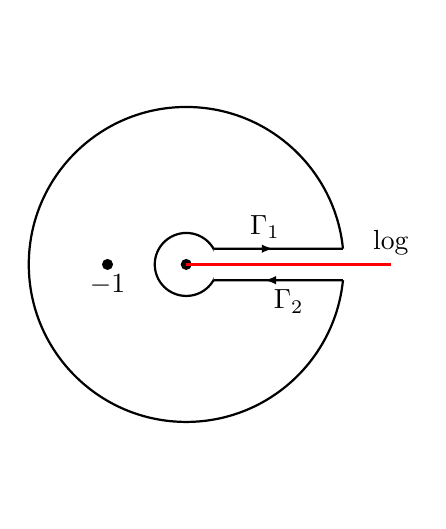
\begin{tikzpicture}[scale=1] 
      \draw[thick, name path=C1] (0,0) circle (2);       
      \draw[thick, name path=C2] (0,0) circle (0.4);
      \fill[black] (0,0) circle (2pt);
      \draw [opacity=0.0, name path=line1] (0,0.2)--(2.1,0.2);       
      \draw [opacity=0.0] (0,-3)--(0,3);        
      \draw [opacity=0.0, name path=line2] (0,-0.2)--(2.1,-0.2);
      \draw [name intersections={of= C1 and line1, by={a}}];
      \draw [name intersections={of= C2 and line1, by={b}}];        
      \draw [name intersections={of= C1 and line2, by={c}}];
      \draw [name intersections={of= C2 and line2, by={d}}];
      \fill [white] (d)--(2.1,-0.2)--(2.1,0.2)--(b)--cycle;
      \draw[thick] (d)--(c);
      \draw[thick] (b)--(a);
      \draw (1.0,0.2) node[above]{$\Gamma_{1}$};        
      \draw (1.3,-0.2) node[below]{$\Gamma_{2}$};
      \fill (-1,0) circle (2pt) node[below] {$-1$};
      \draw [-latex, thin] (b)--(1.1,0.2);
      \draw [-latex, thin] (c)--(1.0,-0.2);
      \draw [red, thick] (0,0)--(2.6,0);
      \draw (2.6,0) node [above]{$\log$};
    \end{tikzpicture}    
    \caption{積分路}
\end{figure}

\begin{figure}[ht]
  \centering    
  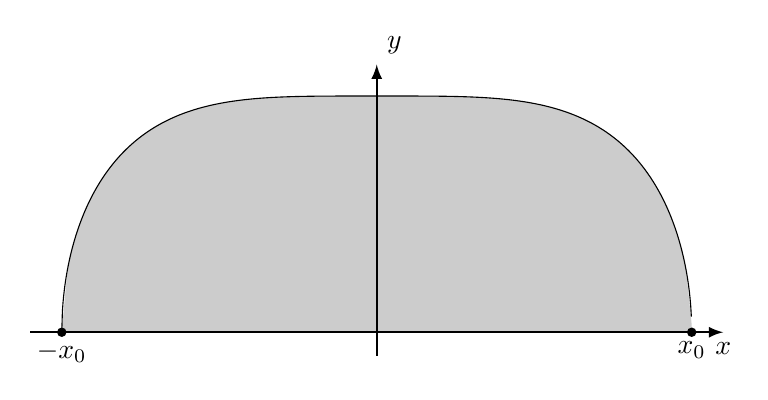
\begin{tikzpicture}[scale=1]       
    \fill[opacity=0.2] plot [smooth,samples=100,domain=-4:4] (\x,{sqrt(abs(4*4*4*4-\x*\x*\x*\x))/16*3}) -- (4,0) -- (-4,0);
    \draw[-latex,thick] (-4.4,0)--(4.4,0) node [below]{$x$};
    \draw[-latex,thick] (0,-0.3)--(0,3.4) node [above right] {$y$};
    \draw[name path=int, domain=-4:4,samples=1000] plot (\x,{sqrt(abs(4*4*4*4-\x*\x*\x*\x))/16*3});
    \fill(-4,0)circle(0.06)node[below]{$-x_0$};
    \fill(4,0)circle(0.06)node[below]{$x_0$};
  \end{tikzpicture}    
  \caption{積分の値}
\end{figure}

\begin{figure}[ht]
  \centering    
  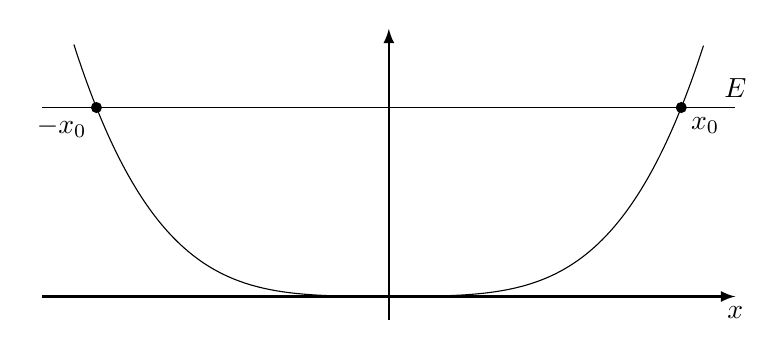
\begin{tikzpicture}[scale=1]
    \draw[-latex,thick] (-4.4,0)--(4.4,0) node [below]{$x$};
    \draw[-latex,thick] (0,-0.3)--(0,3.4);
    \draw[name path=int, domain=-4:4,samples=1000] plot (\x,{(\x*\x+\x*\x*\x*\x)/(4*4+4*4*4*4)*3.2});
    \draw[name path=en, thin] (-4.4,2.4)--(4.4,2.4) node [above] {$E$};
    \path[name intersections={of= int and en, by={a,b}}];
    \fill (a)circle(2pt) node [below left] {$-x_{0}$};
    \fill (b)circle(2pt) node [below right] {$x_{0}$};
  \end{tikzpicture}    
  \caption{ポテンシャル}
\end{figure}

\begin{figure}[ht]
  \centering    
  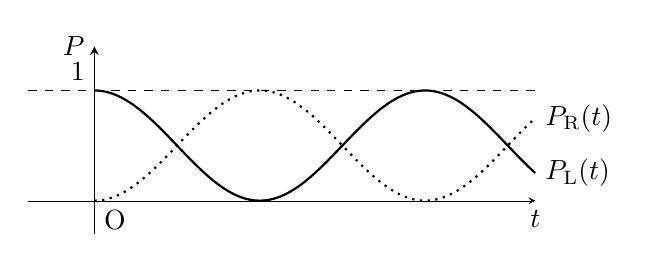
\begin{tikzpicture}[scale=1.4]
      \draw[->,>=stealth,ultra thin](-0.6,0)--(4,0)node[below]{$t$};
      \draw[->,>=stealth,thin](0,-0.3)--(0,1.4)node[left]{$P$};
      \draw(0,0)node[below right]{O};
      \draw[dashed,thin](-0.6,1)--(4,1);
      \draw(0,1)node[above left]{$1$};
      \draw[thick,samples=100,domain=0:4]plot(\x,{(1+cos(\x*360/3))/2})node[right]{$P_{\text{L}}(t)$};
      \draw[thick,samples=100,domain=0:4,dotted]plot(\x,{(1-cos(\x*360/3))/2})node[right]{$P_{\text{R}}(t)$};
    \end{tikzpicture}    
    \caption{$P_{\text{L}}$と$P_{{\text{R}}}$の時間変化}
\end{figure}

\begin{figure}[ht]
  \centering    
  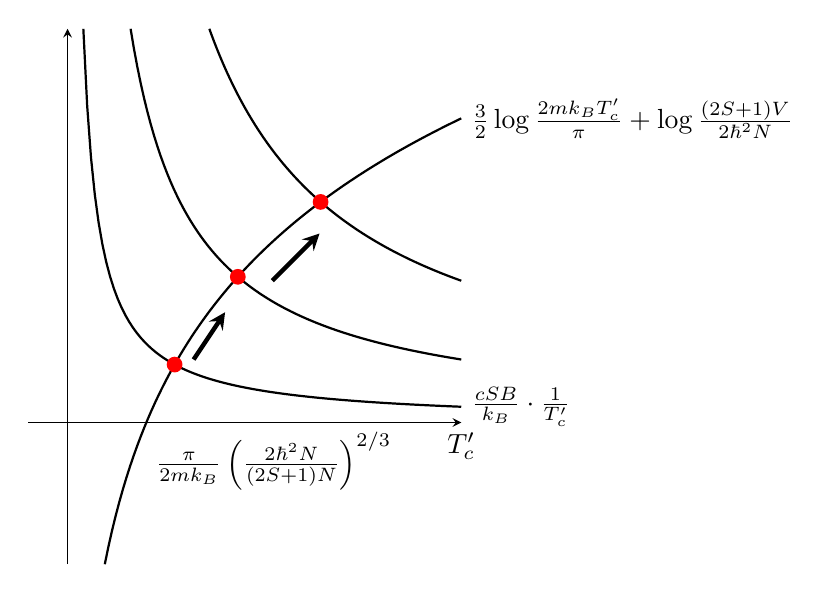
\begin{tikzpicture}
    \draw[->,>=stealth](-0.5,0)--(5.0,0)node[below]{$T_{c}^{\prime}$};
    \draw[->,>=stealth](0,-1.8)--(0,5.0);
    \draw[thick,samples=100,domain=exp(-1.8/2.4):5,name path=A]plot(\x,{2.4*ln(\x)})node[right]{$\frac{3}{2}\log\frac{2mk_{B}T_{c}^{\prime}}{\pi}+\log\frac{(2S+1)V}{2\hbar^2N}$};
    \draw[thick,samples=100,domain=1/5:5,name path=B]plot(\x,{1/(\x)})node[right]{$\frac{cSB}{k_{B}}\cdot\frac{1}{T_{c}^{\prime}}$};
    \draw[thick,samples=100,domain=4/5:5,name path=C]plot(\x,{4/(\x)});
    \draw[thick,samples=100,domain=9/5:5,name path=D]plot(\x,{9/(\x)});
    \path[name intersections={of= A and B, by=E}];
    \path[name intersections={of= A and C, by=F}];
    \path[name intersections={of= A and D, by=G}];
    \fill[red](E)circle(0.1);
    \fill[red](F)circle(0.1);          
    \fill[red](G)circle(0.1);
    \draw[->,>=stealth,ultra thick](1.6,0.8)--(2.0,1.4);
    \draw[->,>=stealth,ultra thick](2.6,1.8)--(3.2,2.4);
    \draw(1,0)node[below right]{$\frac{\pi}{2mk_{B}}\left( \frac{2\hbar^2 N}{(2S+1)N} \right)^{2/3}$};
  \end{tikzpicture}
  \caption{セルフコンシステントに転移温度$T_{c}^{\prime}$を求める方法}    
\end{figure}

\begin{figure}[ht]
  \centering
  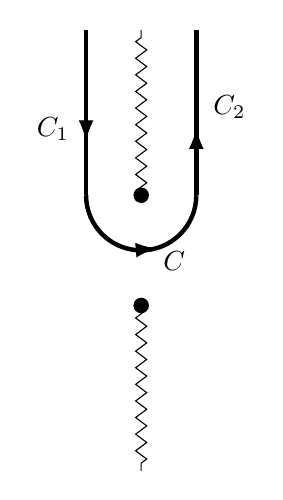
\begin{tikzpicture}[scale=1.4]
    \draw[decorate, decoration={zigzag, segment length=6, amplitude=2}] (0,0.5) -- (0,2);    
    \draw[decorate, decoration={zigzag, segment length=6, amplitude=2}] (0,-0.5) -- (0,-2);
    \fill (0,0.5) circle (2pt);    
    \fill (0,-0.5) circle (2pt);
    \draw[ultra thick] (-0.5,2) -- (-0.5,0.5);
    \draw[ultra thick] (0.5,2) -- (0.5,0.5);
    \draw[-{Latex[length=2.5mm]}](-0.5,1.1)--(-0.5,1.0);
    \draw[-{Latex[length=2.5mm]}](0.5,1.0)--(0.5,1.1);    
    \draw[ultra thick] (-0.5,0.5) arc (180:360:0.5);        
    \draw[-{Latex[length=2.5mm]}] (-0.5,0.5) arc (180:285:0.5);
    \draw (0.3,-0.1) node {$C$};     
    \draw (0.8,1.3) node {$C_{2}$};      
    \draw (-0.8,1.1) node {$C_{1}$}; 
  \end{tikzpicture}
  \caption{変更後の経路}
\end{figure}

\begin{figure}[ht]
  \centering    
  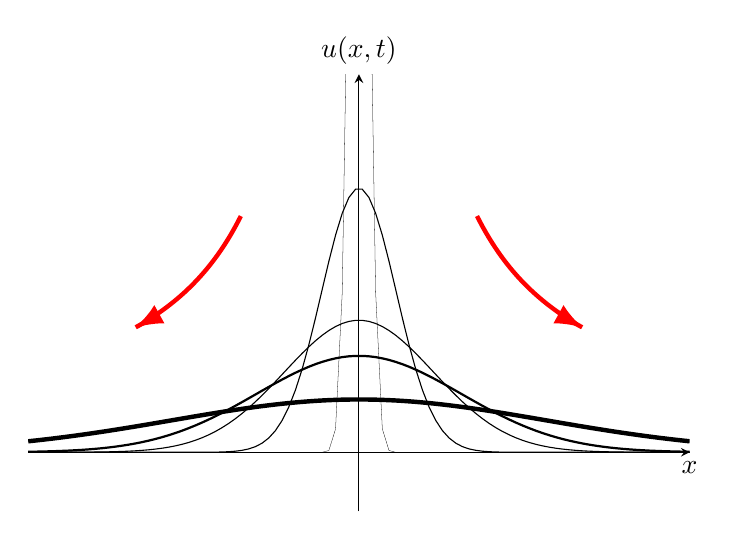
\begin{tikzpicture}[scale=1.5] 
      \draw[->,>=stealth](0,-0.5)--(0,3.2)node[above]{$u(x,t)$};
      \draw[->,>=stealth](-2.8,0)--(2.8,0)node[below]{$x$};
      \draw[-Latex,samples=100,domain=1.0:1.9,ultra thick,red]plot(\x,2/\x);
      \draw[-Latex,samples=100,domain=1.0:1.9,ultra thick,red]plot(-\x,2/\x);
      \begin{scope} \clip (-2.8,-0.5) rectangle (2.8,3.2);
        \draw[samples=100,domain=-2.8:2.8,ultra thin]plot(\x,{exp(-\x*\x/0.01)/sqrt(0.01)});
        \draw[samples=100,domain=-2.8:2.8,thin]plot(\x,{exp(-\x*\x/0.2)/sqrt(0.2)});
        \draw[samples=100,domain=-2.8:2.8]plot(\x,{exp(-\x*\x/0.8)/sqrt(0.8)});
        \draw[samples=100,domain=-2.8:2.8,thick]plot(\x,{exp(-\x*\x/1.5)/sqrt(1.5)});
        \draw[samples=100,domain=-2.8:2.8,ultra thick]plot(\x,{exp(-\x*\x/5)/sqrt(5)});
      \end{scope}
    \end{tikzpicture}    
    \caption{$u(x,t)$の様子}
\end{figure}

\begin{figure}[ht]
  \begin{minipage}[ht]{0.49\columnwidth}
    \centering
    \begin{tikzpicture}
      \draw[thin,-Stealth] (-0.2,0)--(3.5,0)node[above]{$t$};
      \draw[thin,-Stealth] (0,-1.5)--(0,2)node[left]{$x(t)$};
      \draw[very thick,samples=100,domain=0.01:3.5]plot(\x,{exp(-1.2*\x)*(exp(\x)-exp(-\x))});
    \end{tikzpicture}
    \caption{$\beta>\omega$のとき}
  \end{minipage}
  \begin{minipage}[ht]{0.49\columnwidth}
    \centering
    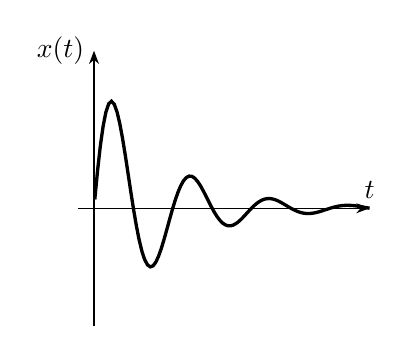
\begin{tikzpicture}
      \draw[thin,-Stealth] (-0.2,0)--(3.5,0)node[above]{$t$};
      \draw[thin,-Stealth] (0,-1.5)--(0,2)node[left]{$x(t)$};
      \draw[very thick,samples=100,domain=0.01:3.5]plot(\x,{1.8*exp(-1.2*\x)*(sin(\x*360))});
    \end{tikzpicture}
    \caption{$\beta<\omega$のとき}
  \end{minipage}    
\end{figure}

\begin{figure}[ht]
  \begin{minipage}[ht]{0.33\columnwidth}
    \centering
    \begin{tikzpicture}
      \draw[thin,-Stealth] (-2,0)--(2,0)node[above]{$\vec{e}^{(1)}$};
      \draw[thin,-Stealth] (0,-2)--(0,2)node[left]{$\vec{e}^{(2)}$};
      \draw[very thick,-latex] (0,0)--(1.3,1.3);        
      \draw[dotted] (-2,-2)--(2,2);
    \end{tikzpicture}
    \caption{$\delta=0$のとき}
  \end{minipage}
  \begin{minipage}[ht]{0.33\columnwidth}
    \centering
    \begin{tikzpicture}
      \draw[thin,-Stealth] (-2,0)--(2,0)node[above]{$\vec{e}^{(1)}$};
      \draw[thin,-Stealth] (0,-2)--(0,2)node[left]{$\vec{e}^{(2)}$};
      \draw[very thick,-latex] (0,0)--(1.2,1.2);        
      \draw[dotted,-latex] (0,0) circle ({1.2*sqrt(2)});
      \draw [-latex] (30:{1.2*sqrt(2)+0.3}) arc [start angle=30, end angle=60, radius={1.2*sqrt(2)+0.3}];
      \draw [-latex] (210:{1.2*sqrt(2)+0.3}) arc [start angle=210, end angle=240, radius={1.2*sqrt(2)+0.3}];
    \end{tikzpicture}
    \caption{$\delta=\pi/2$のとき}
  \end{minipage}
  \begin{minipage}[ht]{0.33\columnwidth}
    \centering
    \begin{tikzpicture}
      \draw[thin,-Stealth] (-2,0)--(2,0)node[above]{$\vec{e}^{(1)}$};
      \draw[thin,-Stealth] (0,-2)--(0,2)node[left]{$\vec{e}^{(2)}$};
      \draw[very thick,-latex] (0,0)--(1.2,1.2);        
      \draw[dotted,-latex] (0,0) circle ({1.2*sqrt(2)});\draw [-latex] (60:{1.2*sqrt(2)+0.3}) arc [start angle=60, end angle=30, radius={1.2*sqrt(2)+0.3}];
      \draw [-latex] (240:{1.2*sqrt(2)+0.3}) arc [start angle=240, end angle=210, radius={1.2*sqrt(2)+0.3}];
    \end{tikzpicture}
    \caption{$\delta=-\pi/2$のとき}
  \end{minipage}
\end{figure}


\begin{figure}[ht]    
  \centering
  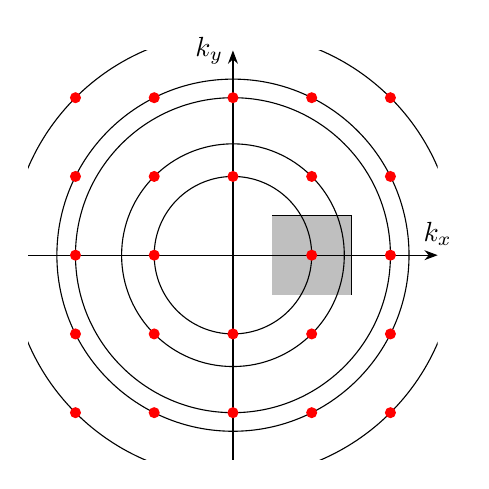
\begin{tikzpicture}
    \draw[thin](0.5,0.5)--(1.5,0.5)--(1.5,-0.5)--(0.5,-0.5)--cycle;
    \fill[lightgray](0.5,0.5)--(1.5,0.5)--(1.5,-0.5)--(0.5,-0.5)--cycle;
    \draw[-Stealth] (-2.6,0)--(2.6,0)node[above]{$k_x$};
    \draw[-Stealth] (0,-2.6)--(0,2.6)node[left]{$k_y$};      
    \begin{scope} \clip (-2.6,-2.6) rectangle (2.6,2.6);
      \draw(0,0) circle (1);
      \draw(0,0) circle ({sqrt(2)});
      \draw(0,0) circle (2);      
      \draw(0,0) circle ({sqrt(5)}); 
      \draw(0,0) circle ({2*sqrt(2)});       
      \fill[red](1,0) circle (2pt);\fill[red](1,1) circle (2pt);\fill[red](1,2) circle (2pt);\fill[red](2,0) circle (2pt);\fill[red](2,1) circle (2pt);\fill[red](2,2) circle (2pt);\fill[red](1,-1) circle (2pt);\fill[red](1,-2) circle (2pt);\fill[red](2,-1) circle (2pt);\fill[red](2,-2) circle (2pt);\fill[red](0,-2) circle (2pt);\fill[red](0,-1) circle (2pt);\fill[red](0,1) circle (2pt);\fill[red](0,2) circle (2pt);\fill[red](-1,0) circle (2pt);\fill[red](-1,1) circle (2pt);\fill[red](-1,2) circle (2pt);\fill[red](-2,0) circle (2pt);\fill[red](-2,1) circle (2pt);\fill[red](-2,2) circle (2pt);\fill[red](-1,-1) circle (2pt);\fill[red](-1,-2) circle (2pt);\fill[red](-2,-1) circle (2pt);\fill[red](-2,-2) circle (2pt);
    \end{scope}
  \end{tikzpicture}
  \caption{$(k_x,k_y)$の取りうる値}
\end{figure}


\begin{figure}[ht]    
  \centering
  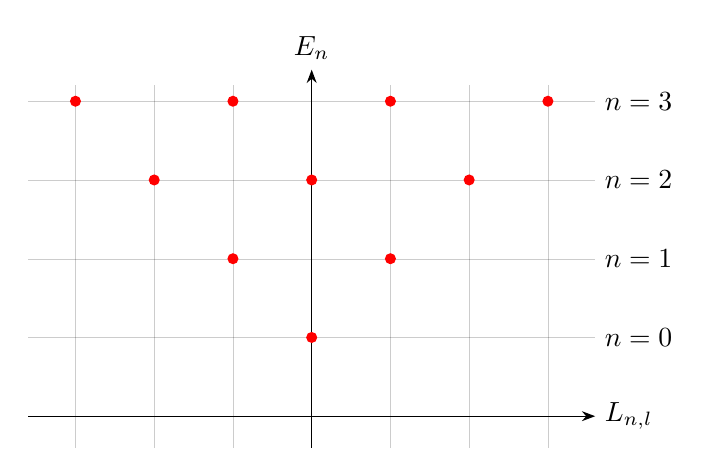
\begin{tikzpicture}
    \draw[-Stealth] (-3.6,0)--(3.6,0)node[right]{$L_{n,l}$};
    \draw[-Stealth] (0,-0.4)--(0,4.4)node[above]{$E_n$};      
    \begin{scope} \clip (-3.6,-0.4) rectangle (3.6,4.2);
      \draw[ultra thin, opacity=0.2] (1,-0.4)--(1,4.2);
      \draw[ultra thin, opacity=0.2] (2,-0.4)--(2,4.2);
      \draw[ultra thin, opacity=0.2] (3,-0.4)--(3,4.2);
      \draw[ultra thin, opacity=0.2] (-1,-0.4)--(-1,4.2);
      \draw[ultra thin, opacity=0.2] (-2,-0.4)--(-2,4.2);
      \draw[ultra thin, opacity=0.2] (-3,-0.4)--(-3,4.2);
      \draw[ultra thin, opacity=0.2] (-3.6,1)--(3.6,1);
      \draw[ultra thin, opacity=0.2] (-3.6,2)--(3.6,2);
      \draw[ultra thin, opacity=0.2] (-3.6,3)--(3.6,3);
      \draw[ultra thin, opacity=0.2] (-3.6,4)--(3.6,4);
    \end{scope}
    \draw(3.6,1)node[right]{$n=0$};
    \draw(3.6,2)node[right]{$n=1$};
    \draw(3.6,3)node[right]{$n=2$};
    \draw(3.6,4)node[right]{$n=3$};
    \fill[red](0,1)circle(2pt);
    \fill[red](1,2)circle(2pt);
    \fill[red](-1,2)circle(2pt);
    \fill[red](0,3)circle(2pt);
    \fill[red](2,3)circle(2pt);
    \fill[red](-2,3)circle(2pt);
    \fill[red](-3,4)circle(2pt);
    \fill[red](-1,4)circle(2pt);
    \fill[red](1,4)circle(2pt);
    \fill[red](3,4)circle(2pt);
  \end{tikzpicture}
  \caption{設問8の答え}
\end{figure}

\begin{figure}[ht]
  \centering
  \begin{tikzpicture}[scale=1.5]
    \draw[thin,-Stealth] (0,0)--(3.5,0)node[right]{$\omega$};
    \draw[thin,-Stealth] (0,0)--(0,3.5)node[left]{$n^2(\omega)$};   
    \draw[dotted,thin] (3.5,1.5)--(0,1.5)node[left]{1};
    \draw[dotted,thin] (1.2,3.5)--(1.2,0)node[below]{赤};
    \draw[dotted,thin] (2.5,3.5)--(2.5,0)node[below]{紫};
    \draw[thick,Stealth-Stealth] (1.2,3.5)--(2.5,3.5);
    \draw[dotted,thin] (1.7,3.5)--(1.7,0)node[below]{$\omega_0$};
    \begin{scope} \clip (0,0) rectangle (3.5,3.5);
      \draw[samples=100,domain=0:1.65,thick]plot(\x,{1.7-(1)/((1.7)^2)+(1)/(-(\x)^2+(1.7)^2)});        
      \draw[samples=100,domain=1.75:3.5,thick]plot(\x,{1.7-(1)/((1.7)^2)+(1)/(-(\x)^2+(1.7)^2)});           
    \end{scope}
  \end{tikzpicture}
  \caption{物質Fの分散曲線}
\end{figure}

\begin{figure}[ht]
  \centering    
  \begin{tikzpicture}[scale=1.6] 
    \draw[->,>=stealth,thin](-0.2,0)--(3,0)node[below]{$x$};
    \draw[->,>=stealth,thin](0,-0.5)--(0,2.0);
    \begin{scope} \clip (-0.2,-0.5) rectangle (3,2);
      \draw[samples=100,domain=0.1:3,thick]plot(\x,{1.1*(exp(-1*(\x)-exp(-2*(\x))))/(\x)});        
    \end{scope}
  \end{tikzpicture}    
  \caption{$\ev*{\bm{x}|\psi}$の概形}
\end{figure}


\begin{figure}[ht]
  \centering    
  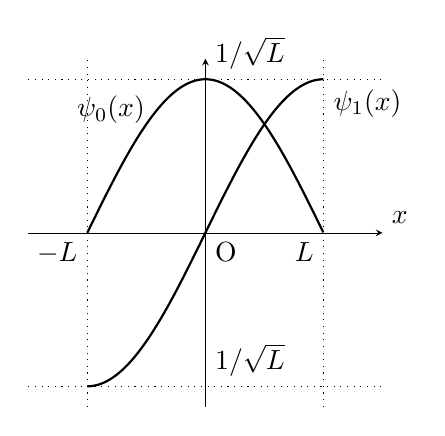
\begin{tikzpicture}[xscale=1.5, yscale=1.3]
    \draw[->,>=stealth,ultra thin](0,-1.7)--(0,1.7);
    \draw[->,>=stealth,ultra thin](-1.5,0)--(1.5,0)node[above right]{$x$};
    \draw[dotted,thin](1,-1.7)--(1,1.7);
    \draw[dotted,thin](-1,-1.7)--(-1,1.7);
    \draw[dotted,thin](-1.5,-1.5)--(1.5,-1.5);
    \draw[dotted,thin](-1.5,1.5)--(1.5,1.5);
    \draw(0,0)node[below right]{O};
    \draw(1,0)node[below left]{$L$};
    \draw(-1,0)node[below left]{$-L$};
    \draw[samples=100,domain=-1:1,thick]plot(\x,{1.5*(cos(\x*90))}); 
    \draw[samples=100,domain=-1:1,thick]plot(\x,{1.5*(sin(\x*90))}) node[below right]{$\psi_1(x)$}; 
    \draw(-0.8,1.2)node{$\psi_0(x)$};
    \draw(0,1.5)node[above right]{$1/\sqrt{L}$};
    \draw(0,-1.5)node[above right]{$1/\sqrt{L}$};
  \end{tikzpicture}
  \caption{$\psi_0(x)$と$\psi_1(x)$の概形}
\end{figure}

\begin{figure}[ht]
  \centering    
  \begin{tikzpicture}[scale=2.0]
    \draw[->,>=stealth,ultra thin](0,-0.3)--(0,1.8);
    \draw[->,>=stealth,ultra thin](-0.3,0)--(2.0,0)node[below right]{$V_1$};
    \draw[dotted,thin](-0.3,1.5)--(2.0,1.5)node[right]{$E_1$};
    \draw[samples=100, domain=0.0:2.0, thick]plot(\x,{1.4-exp(-2*\x)});
    \draw(0.4,0.6) node{$E_0$};
  \end{tikzpicture}
  \caption{$E_0$と$E_1$}
\end{figure}

\end{document}
